%%%%%%%%%%%%%%%%%%%% author.tex %%%%%%%%%%%%%%%%%%%%%%%%%%%%%%%%%%%
%
% sample root file for your "contribution" to a proceedings volume
%
% Use this file as a template for your own input.
%
%%%%%%%%%%%%%%%% Springer %%%%%%%%%%%%%%%%%%%%%%%%%%%%%%%%%%


\documentclass{svproc}
%
% RECOMMENDED %%%%%%%%%%%%%%%%%%%%%%%%%%%%%%%%%%%%%%%%%%%%%%%%%%%
%

% to typeset URLs, URIs, and DOIs
\usepackage{url}
\usepackage{graphicx}
\graphicspath{ {images/} }
\def\UrlFont{\rmfamily}

\begin{document}
\mainmatter              % start of a contribution
%
\title{A system to facilitate the mobility of visually impaired people}
%
\titlerunning{capTeus - CAPtiosus balTEUS}  % abbreviated title (for running head)
%                                     also used for the TOC unless
%                                     \toctitle is used
%
\author{Gleiston Guerrero-Ulloa\inst{1} \and Henry Perez-Mu\~{n}oz \and
Efra\'{i}n D\'{i}az-Mac\'{i}as \and Orlando Erazo Moreta}
%
\authorrunning{Gleiston Guerrer-Ulloa et al.} % abbreviated author list (for running head)
%
%%%% list of authors for the TOC (use if author list has to be modified)
\tocauthor{Gleiston Guerrero-Ulloa\inst{1}, Henry Perez-Mu\~{n}oz, Efra\'{i}n D\'{i}az-Mac\'{i}as, Orlando Erazo Moreta}
%
\institute{Universidad Técnica Estatal de Quevedo, Quevedo Los Ríos 120301, Ecuador,\\
\email{\{gguerrero, henry.perez2017, efraindiaz, oerazo\}@uteq.edu.ec},\\
WWW home page: \texttt{https://www.uteq.edu.ec/}
}

\maketitle              % typeset the title of the contribution

\begin{abstract}
The number of visually impaired persons (VIP) who move
around alone is growing day by day. This has increased the concern of
responsible persons (relatives) for their well-being. Some solutions have
been presented that help both VIP to move more safely and their families
to be more relaxed. Our contribution is a prototype called CapTeus,
which can alert blind people and give them indications to evade obstacles
in their path. In addition, relatives will be able to receive text messages
or messages to Telegram. CapTeus has been developed using the
Test-Driven Development Methodology for IoT-based Systems. Obstacle
recognition has been performed at a maximum of 200cm, and Google’s
TensorFlow API has been used, obtaining an accuracy to 100\%, depending
on the obstacle and the distance. The evaluation of this prototype was
carried out with VIP in real and controlled scenarios. CapTeus achieved
a 96\% acceptance rate among users.
\keywords{obstacle recognition, visually impaired, Internet of things, Test-Driven Development}
\end{abstract}
%
\section{Introduction}
%
There are about 2.2 billion people with visual impairment (VIP) in the world. Of
these, 14.50\% suffer from moderate blindness, 16.69\% suffer from moderate to
severe blindness and 2.77\% are blind \cite{Pan2023}. In Ecuador, according to data provided
by the National Council for Equality of Disabilities (acronym in Spanish CONADIS), by mid-2022
there were 54,397 VIP, either from birth or due to disease, representing 11.54\% of
the total number of people with disabilities in Ecuador \cite{conadis2023}. The inclusion of these
people starts at home, so their families must provide them with some strategy
to help them become self-sufficient in their mobilization, without neglecting the
safety of the VIP or the peace of mind of them.

VIPs often use white canes or guide dogs in their mobilization, and face
adversity along the way. Unfortunately, these resources can be ineffective in
adequately alerting them to dangers in their path. Similarly, they are unable to
help a VIP recognize obstacles, especially those who are new to the disability or
their training. On a path, people may encounter obstacles such as signs, electric
lighting poles, fire hydrants or trees, among others \cite{Vorapatratorn2015}. Guide dogs are usually one of the most viable options for the mobilization of VIPs, but there is a possibility
that during their trajectory they may coincide with untrained dogs, which may
cause the VIP to be at risk due to confrontations between canines \cite{Vorapatratorn2015,Hertel2019}.

Moreover, the acquisition of a trained guide dog entails a significant upfront
expenditure of approximately US\$50,000 \cite{Williams2020}, along with its consequent maintenance
and everyday upkeep costs. Nonetheless, the precise outlay is subject to
regional disparities in training practices, such that the initial cost of training a
guide dog in Ecuador amounts to US\$12,000 US dollars, accounting for a training
period of no more than one year and an anticipated work span of nearly a dozen
years \cite{EPGE}. Therefore, it is necessary to look for accessible, safe and comfortable
alternatives for this segment of the population.

Currently, technologies such as the Internet of Things (IoT) make it possible
to build intelligent devices, interconnecting physical objects through the Internet.
IoT aims to help improve people’s lifestyle. For example, VIPs can detect
and recognize objects \cite{Leporini2022}, being able to improve their daily life by trying to
improve their self-sufficient life \cite{Gupta}.

Leveraging IoT technologies, accessible solutions for VIP have been implemented.
Vorapatratorn and Teachavorasinskun \cite{Vorapatratorn2017} present a solution consisting
of an ear accessory connected to a device that goes on the user’s waist. It allows
identifying obstacles at 130 cm and alerting the user by emitting vibrations.
Vorapatratorn and Teachavorasinskun \cite{Vorapatratorn2017} take into account the recognition of
objects so that the user can make the best decisions and avoid them. Another
work with similar functions can be considered the work of Kazi et al. \cite{Kasi2023} developed
an smart cane capable of detecting obstacles and recognizing their type.
Although the user can have several types of outputs (depending on his or her
disability) to guide him or herself, it does not provide for communication with a
family member in case of emergency. None of these documents mention the functionality
of the device to allow the user to communicate with his/her relatives
in case of emergency.

\section{Related Works}

The inclusion of people with disabilities in society and in the world of work has
allowed them to learn to be self-sufficient, and to move around to meet their
daily obligations/needs. These changes have increased the concern of academics
to develop solutions for these people to move around more safely and for their
relatives to remain more at ease when they are away from them. In the case
of the visually impaired, some very promising solutions have been developed,
although none fully meet the needs of the users. Among those solutions, one
can cite the work of Hertel \cite{Hertel2019}, in which they propose the design of a cane
device called STIC, which assists the mobility of a VIP by making use of an
ultrasonic distance sensor for head level and a laser-based infrared sensor for
ground level obstacle detection. Feedback to user on obstacle detection is encoded
and transmitted through vibrotactile actuators. Thus, the VIP must learn to
perceive the intensity of vibrations to identify the distance of the obstacle in
front of it.

On the other hand, Rajesh et al. \cite{Rajesh2023}, present a system in which they have
used a buzzer and multiple ultrasonic sensors with which they try to give security
on the way to the VIP. The sensors are used to detect obstacles and stairs, and
the humidity of the ground to issue an alert according to the situation. It also
allows to know the location of the blind person using the cell phone, to be used as
part of an emergency message that can be sent to the cell phones of the specified
numbers.

Another work that combines ultrasonic obstacle detection sensors to make
the blind person’s trajectory more comfortable is SCBIoT presented by AbdElminaam
et al. \cite{AbdElminaam2022}. In addition to obstacle detection, SCBIoT uses a GPS
module to send a periodic mail with the user’s location by connecting to the Wi-
Fi hotspot of the Android phone. This way you can keep your family members
informed. In addition, they incorporate vibrators and a buzzer that try to help
and warn the user of any obstacle.

The work of Rajesh et al. \cite{Rajesh2023}, the user must learn the meaning of the alerts he
receives by vibration and sound. In addition, in the work of AbdElminaam et
al. \cite{AbdElminaam2022}. when trying to keep family members informed by e-mail, it may happen
that they are not attentive, and when they check their e-mail it is too late. The
works of AbdElminaam et al. \cite{AbdElminaam2022}. as well as Rajesh et al. \cite{Rajesh2023} are very promising, however it can be considered that users may be distressed by not recognizing
the obstacle in front of them, as they only detect them.

In addition to canes to assist VIPs, smart shoes have been developed, such as
the work of Nathan el al. \cite{Nathan2023}. The shoes are equipped with sensors and actuators
to detect obstacles and inform VIPs, trying to make them walk autonomously.
In addition to an emergency fall notification through a buzzer and speakers (DF
Player) so that people nearby can help the VIP, while their relatives are notified
through \cite{Blynk2023}. Likewise, the smart shoe designed by Suneetha et al. \cite{Suneetha}
offers a possible solution for blind people to walk on the street independently.
This shoe, like the one proposed by Nathan et al. \cite{Nathan2023}, has several built-in sensors,
a microcontroller and buzzers, with the difference that the one by Suneetha et
al. \cite{Suneetha} only warns by a buzzer when there is an obstacle in front of the VIP.

Both canes and shoes detect obstacles uniquely, with the exception of Rajesh et al. \cite{Rajesh2023}
s work which identifies obstacles as Large, Medium and Small. The limitations of the works retrieved and reviewed in this paper have inspired the authors of this work to propose CapTeus as a prototype that allows to detect and recognize obstacles in the way of the VIP, and is equipped with a panic
button (as is the work of Rajesh et al. \cite{Rajesh2023}) to notify in case of emergencies to their relatives via Telegram messages and emails, or text messages when they
do not have internet connection.

\section{CapTeus: The Proposed System}

CapTeus (Latin: \textit{cap}tiosus bal\textit{teus}) is proposed as a viable solution to guide blind
people in their daily walks. CapTeus is an economically viable system with high
usability acceptance. It was built and tested with real user requirements. Capteus
can detect obstacles, recognize them, warn the user about them and guide the
user where to go to avoid the obstacle. In addition, in case of emergency, the
user carrying the device can press a panic button to inform relatives about the
situation via Telegram message and emails, or in case of no internet connection
via SMS. CapTeus consists of a device and a mobile application.

\subsection{Obstacle Detection Method}

Obstacle detection is performed by the reflection of ultrasonic waves transmitted
by an ultrasonic sensor. The distance is given by the time it takes for the wave
to return multiplied by the speed of sound divided by two.

\subsection{Obstacle Recognition Method}

Recognizing obstacles through artificial intelligence after encountering and identifying
them is vital for a VIP to know what is in front of it when following a
path, especially in open environments. This is the reason why this important
functionality was implemented in CapTeus. In the realization of CapTeus, the
TensorFlow Lite API is used, which is focused on the use of mobile devices,
has a comprehensive and flexible ecosystem of tools, libraries and community
resources; which allows researchers to innovate with machine learning and developers
to create and implement applications with DL technology \cite{Google}.

\subsection{TensorFlow}
CapTeus uses TensorFlow for obstacle recognition. It is an open source API for
Deep Learning (DL). This API allows building and training neural networks to
detect patterns and reason like humans. They are used for object recognition,
image classification, among others. TensorFlow is ideal for CapTeus because
it covers from mobile devices such as smartphones and tablets to large-scale
distributed systems and other computational devices [17].

\subsection{Issuance of Notifications for the VIP}

CapTeus issues notifications to the VIP by voice. The texts of the notifications
are formed based on the obstacle about which the VIP needs to be notified.
Once the text is obtained, it is converted to speech using an Android class called
Text-to-Speak, which receives the text and the information is obtained as a result
through the smartphone’s synthesizers \cite{Tufan2022}.

\section{Development Methodology of CapTeus}

For the development of CapTeus, the Test-Driven Methodology for IoT-based
Systems (TDDM4IoTS) \cite{Guerrero-Ulloa2020} has been used, as it is an agile methodology and
one of those that best covers the life cycle of the systems in its phases \cite{Guerrero-Ulloa2023}.
TDDM4IoTS is a methodology which consists of 11 phases: preliminary analysis,
tecnology layer design, detailed requirement analysis, model generation and
adaptation, test generation, software generation, model refinement, software refinement,
hardware and software deployment, deliverable assessment, maintenance
\cite{Guerrero-Ulloa2020}. TDDM4IoTS focuses specifically on the development of IoT-based
systems \cite{Guerrero-Ulloa2020,Guerrero-Ulloa2023}.

TDDM4IoTS is a flexible methodology, in which the order of the phases and
the phases themselves are not a straitjacket. Developers decide which ones should
be executed and in what order \cite{Guerrero-Ulloa2020}. For this, it is necessary to observe the type of project, the experience of the project team in the development of this type of
projects, among other aspects.

\subsection{Execution of the TDDM4IoTS Phases in the Development of CapTeus}

For example, the maintenance phase because CapTeus is a prototype in the testing
phase. Also, the model and software refinement phase because it was a system
whose requirements were clear and the software code was written manually with
clean code best practices.

\subsubsection{Preliminary Analysis.} In this phase, a coarse-grained analysis was performed
to obtain the main functional and non-functional requirements of CapTeus. Technical
aspects such as available tools and technologies, expert personnel in the
development of this type of systems, time available for its development, including
its evaluation, were taken into account to determine whether the development
of CapTeus was feasible or not (\textit{\textbf{technical analysis}}). Being a wearable device, it must have a battery to power it, connected to a mobile Internet signal, among other non-functional requirements (\textit{\textbf{environment analysis}}).

\begin{figure}[h!]
	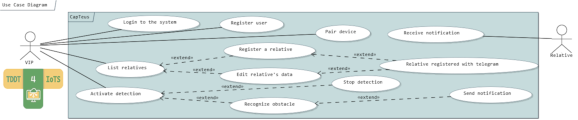
\includegraphics[scale=1.25]{fig1.pdf}
	\centering
	\caption{CapTeus use case diagram.}
	\label{fig:fig1}
\end{figure}

\noindent
\textbf{\textit{Requirements analysis.}} The most important deliverables developed were the following:
User registration, registration of a relative or caregiver, device communication
with the mobile application, obstacle detection, obstacle recognition,
issuance and playback of alerts to the VIP, issuing and Sending Text Message
Notification, broadcasting and sending notification by Telegram.\\

\noindent
\textbf{\textit{Feasibility analysis.}} Regarding the tools and technologies required for its development, there are
many free tools, with many functionalities that facilitate and accelerate the
development of IoTS. The development of CapTeus was done using TDDT4IoTS
as a modeling tool, both for the software and the design of the IoT device. To
program the operation of the mobile application, Android Studio was used as
IDE and Kotlin as programming language, for the SQLite data storage. In terms of economics, its development was feasible, since the only investment
that had to be made was around US\$50. In addition, the simplicity of the activities
that must be performed to keep it operational (on and off, charging its battery,
attaching it to the VIP belt), made it operationally feasible.

\subsubsection{Technology Layer Design.} Considering both software and hardware for fulfilling the functional and nonfunctional requirements of CapTeus, appropriate technologies were sought for alerts in detecting and recognizing obstacles in the VIP trajectory, and sending notifications about the status of the VIP to its family members. These technologies are shown in figure 2, which shows the CapTeus system architecture.

\begin{figure}[h!]
	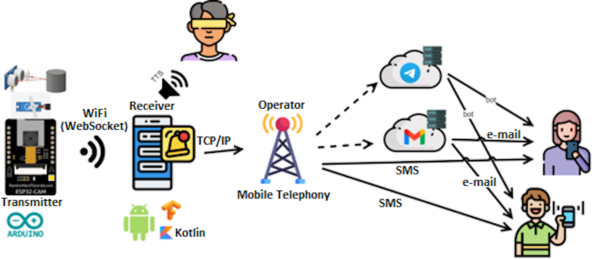
\includegraphics[scale=1.2]{fig2.pdf}
	\centering
	\caption{CapTeus architecture.}
	\label{fig:fig2}
\end{figure}

Figure 3 shows an interconnection diagram of the CapTeus device components.
a) 5-volt battery power supply, b) servo motor to rotate the camera in
search of an alternative path, c) Arduino board to program the rest of the device
components, d) ultra sound sensor to determine the presence of an obstacle and
its distance from the VIP, e) ESP32-CAM camera sensor to capture the image
of the obstacles to be processed for recognition, and f) the button that the PIV
can press when it is in danger. It is one of the diagrams that have been produced
using the TDDT4IoTS tool \cite{Guerrero-Ulloa2021}.

\begin{figure}[h!]
	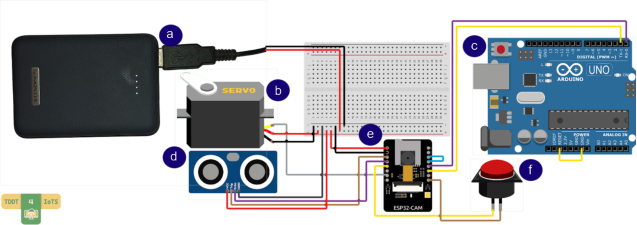
\includegraphics[scale=1.1]{fig3.pdf}
	\centering
	\caption{CapTeus device design.}
	\label{fig:fig3}
\end{figure}

\subsubsection{Detailed Requirement Analysis.} CapTeus requirements are identified in more detail. The modeling of the software architecture was performed obtaining the following artifacts: use case diagram, extended use cases, class diagram, among others. These diagrams were created
using the same TDDT4IoTS tool.

\subsubsection{Model Generation.} The CapTeus class diagram was generated after writing the extended (detailed) use cases using SLUML. The class diagram is shown in figure 4.

\begin{figure}[h!]
	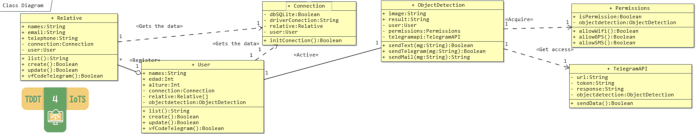
\includegraphics[scale=1.05]{fig4.pdf}
	\centering
	\caption{CapTeus class diagram.}
	\label{fig:fig4}
\end{figure}

\subsubsection{Test Generation.} The generation of tests as a phase of TDDM4IoTS allowed assuring the quality of the developed system. Tests applied were of two types:

\begin{itemize}
	\item Tests performed by the developers: unit tests and integration tests.
	\item Tests performed by a VIP: usability tests, including functional tests.
\end{itemize}

Therefore, the tests performed allowed to ensure that the system complies
with the functionalities according to the established requirements, for each of the
deliverables that were developed in each iteration as specified by TDDM4IoTS.

\subsubsection{Software Generation}
The software for the mobile application was generated 100\% percent manually.
While the software for programming the Arduino board, about 40\% was done
using the TDDTT4IoTS tool. For the writing of the code, the generation of a
clean code was considered to guarantee its maintainability and scalability.

\subsubsection{Model and Software Refinement.}
Being a project with little breadth and complexity, these two phases were not
necessary to be executed, since once the models were generated from the clear
functional requirements, and then the software with good clean code practices.
In addition, the project team has experience in the development of this type of
systems, which helped to accelerate the development of CapTeus.

\subsubsection{Hardware and Software Deployment.}
The hardware and software of the system were deployed in the environment
for which it was built. In this case, since it is a wearable system, its operation
was tested by placing the device on the belt of a VIP and installing the mobile
application on her smartphone, and it was verified that the system works and
interacts with the VIP properly.

\subsubsection{Deliverable assessment.} Once the evaluation by the development team of each deliverable was completed,and finally the integration tests, an assessment was carried out with a group of 27 visually impaired users to assess the performance of the device and the mobile
application in different situations.

The assessment by the VIPs was carried out in two groups. The first group (Group 1) in the province of Los R\'{i}os (La Man\'{a} and Quevedo), and the second
group (Group 2) in the province of Guayas (Guayaquil) in Ecuador. The evaluations
with Group 1 were in controlled environments in which some obstacles
such as chairs, tables, and people were asked to collaborate as obstacles, and
Group 2 in the facilities of the ”Fundaci\'{o}n Ecuatoriana para Ciegos (FUNECI)”
(Ecuadorian Foundation for the Blind). Regarding the acceptance to use or not
to use the device, 74\% totally agree, 22\% agree and 4\% showed some objection
to use it. It should be noted that the effective distance for successful obstacle
recognition is directly proportional to the size of the obstacles.

The more complete the object captured by the camera, the more likely it
is to be recognized. At a distance of 150cm, some objects were not recognized
correctly. Results were obtained from 20\% to 100\% of correctly recognized objects.
The results are shown in the graph in the figure \ref{fig:fig5}.

\begin{figure}[h!]
	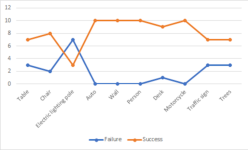
\includegraphics[scale=2]{fig5.pdf}
	\centering
	\caption{Success in obstacle recognition.}
	\label{fig:fig5}
\end{figure}

\section{Conclusions and Future Work}
A cost-effective and user-friendly system has been proposed in this paper. According
to the System Usability Scale (SUS) questionnaire applied to VIPs who
used the system, CapTeus achieved an acceptance rate of 70\%, with a standard
deviation of 7.52. According to Bangor, CapTeus has a good level of acceptance.

Future work includes reducing the size of the CapTeus box. In addition, it is
intended to implement sensors to detect obstacles at ground level (unevenness
of the street or stairs) and sensors to detect the presence of water (humidity or
mud). These sensors could be implemented in a cane or in the VIP’s footwear.

%
% ---- Bibliography ----
%
\begin{thebibliography}{6}
%
\bibitem{Pan2023}
Pan American Health Organization. Visual Health - OPS/OMS. \url{https://www.paho.
org/es/temas/salud-visual}. (Accessed Jan. 27, 2023).

\bibitem{conadis2023}
National Council for Disability Equality. Disability Statistics (2022). \url{https://
www.consejodiscapacidades.gob.ec/estadisticas-de-discapacidad/}. (Accessed Jan. 27, 2023).

\bibitem{Vorapatratorn2015}
Vorapatratorn, S., Teachavorasinskun, K., Chanwarapha, N., Suchato, A. Punyabukkana,
P.: Directional Obstacle Warning Device Using Multiple Ultrasonic
Transducers for People with Visual Disabilities. In: 9th International Convention
on Rehabilitation Engineering \& Assistive Technology, i-CREATe 2015, pp. 1?4.
Singapore Therapeutic, Assistive \& Rehabilitative Technologies (START) Centre,
Midview City, Singapore (2015).

\bibitem{Hertel2019}
Hertel, J., Schaare, A., Feuerbach, P., Ariza, O., Steinicke, F.: STIC - Sensory and
tactile improved cane. In: ACM International Conference Proceeding Series, pp. 765–769. ACM, Hamburg Germany (2019). \url{doi:10.1145/3340764.3344905}.

\bibitem{Williams2020}
Williams, E., Cleghern, Z., Foster, M., Holder, T., Roberts, D., Bozkurt, A.: A Smart
Collar for Assessment of Activity Levels and Environmental Conditions for Guide
Dogs. In: Annual International Conference of the IEEE Engineering in Medicine
and Biology Society. EMBS, vol. 2020-July, pp. 4628?4631. IEEE, (2020). \url{doi:10.1109/embc44109.2020.9175814}.

\bibitem{EPGE}
EPGE: Ecuadorian Guide Dog School. Frequently Asked Questions \url{https://
www.perrosguiaecuatorianos.org.ec/preguntas-frecuentes/}. (Accessed Jan. 02, 2023).

\bibitem{Leporini2022}
Leporini, B., Rosellini, M., Forgione, N.: HapticWearable System to Assist Visually-Impaired People in Obstacle Detection. In: ACM International Conference Proceeding
Series, pp. 269–272. ACM, Corfu Greece (2022). \url{doi:10.1145/3529190.3529217}.

\bibitem {Gupta}
Gupta, D., Rani, S., Raza, S., Faseeh Qureshi, N. M., Mansour, R. F., Ragab, M.:
Security paradigm for remote health monitoring edge devices in internet of things.
Journal of King Saud University - Computer and Information Sciences. In Press
(2023). \url{doi:10.1016/j.jksuci.2022.12.020}.

\bibitem {Vorapatratorn2017}
Vorapatratorn S., Teachavorasinskun, K.: ISonar-2: Obstacle Warning Device, the
Assistive Technology Integrated with Universal Design for the Blind. In: 11th International
Convention on Rehabilitation Engineering and Assistive Technology, in i-CREATe 2017. Midview City, SGP: Singapore Therapeutic, Assistive \& Rehabilitative Technologies (START) Centre, Singapore (2017).

\bibitem {Kasi2023}
Kazi, W., and Limu, T. J., Rakibuzzaman, Md.: Smart Cane: A Low Cost Assistive
Device for the Visually Impaired. EAI Endorsed Transactions on Internet of Things.
8(4), 1?5 (2023). \url{doi:10.4108/eetiot.v8i4.1707}.

\bibitem {Rajesh2023}
Rajesh, P., Sairam, R., Kumar, M. D., Eswar, P. K., Keerthi, Y.: Arduino based
Smart Blind Stick for People with Vision Loss. In: 7th International Conference
on Computing Methodologies and Communication, ICCMC 2023, pp. 1501-1508.
IEEE, Erode, India (2023). \url{doi:10.1109/ICCMC56507.2023.10083752}.

\bibitem {AbdElminaam2022}
AbdElminaam, D. S., Ahmed, I. A. -E., Sakr, F.: SCBIoT: Smart Cane for Blinds
using IoT. In: 2nd International Mobile, Intelligent, and Ubiquitous Computing
Conference, MIUCC 2022, pp. 371-377, IEEE, Cairo, Egypt (2022). \url{doi:10.1109/MIUCC55081.2022.9781728}.

\bibitem {Nathan2023}
Nathan, S. S., Ying, K. J., Wen, L. H., Weoi, L. X.: Design of Smart Walking Shoe
for Visually Impaired People. Journal of Advanced Research in Applied Mechanics,
101(1), 53–61 (2023). \url{doi:10.37934/araset.101.1.5361}.

\bibitem {Blynk2023}
Blynk for Developers. \url{https://blynk.io/developers}. (Accessed January 01, 2023).

\bibitem{Suneetha}
Suneetha, I., Sandhya, A., Rama, L., Reddy, K., Reddy Jyothika, H., Tharun,
C.: Smart Shoe for the Visually Impaired Using IoT. International Journal of
Advances in Engineering and Management, 5(4), 611-614 (2023). \url{doi:10.35629/5252-0504611614}.

\bibitem {Google}
Google Brain Team: TensorFlow, (2022). \url{https://www.tensorflow.org/?hl=es-419}. (Accessed Jul. 01, 2022).

\bibitem {Singh2020}
Singh P., Manure, A.: Introduction to TensorFlow 2.0. Learn TensorFlow 2.0, pp.
1–24 (2020). \url{doi:10.1007/978-1-4842-5558-2_1}.

\bibitem {Tufan2022}
Tufan, B. H. How to use Text to Speech in Android.  \url{https://thecodeprogram.com/how-to-use-text-to-speech-in-android}. (Accessed Jul. 15,
2022).

\bibitem {Guerrero-Ulloa2020} 
Guerrero-Ulloa, G., Hornos, M. J., Rodr\'{i}guez-Dom\'{i}nguez, C.: TDDM4IoTS: a
test-driven development methodology for Internet of Things (IoT)-based systems.
In: Botto-Tobar, M., Zambrano Vizuete, M., Torres-Carri\'{o}n, P., Montes Le\'{o}n,
S., Pizarro V\'{a}squez,G., Durakovic, B. (eds.) Applied Technologies: First International
Conference, ICAT 2019. CCIS, vol 1193, pp. 41?45. Springer, Cham (2020).
\url{doi.org/10.1007/978-3-030-42517-3_4}.

\bibitem {Guerrero-Ulloa2023}
Guerrero-Ulloa, G., Rodr\'{i}guez-Dom\'{i}nguez, C., Hornos, M. J.: Agile Methodologies
Applied to the Development of Internet of Things (IoT)-Based Systems: A Review.
Sensors 23(2), 790-724 (2023). \url{doi:10.3390/s23020790}.

\bibitem {Guerrero-Ulloa2021}
Guerrero-Ulloa, G., Carvajal-Su\'{a}rez, D., Brito-Casanova, G., Pachay-Espinoza, A.:
TDDT4IoTS: Test-Driven Development Tool for IoT-based Systems. (2021). \url{http://www.tddt4iots.tech/}. (Accessed Apr. 15, 2023).

\end{thebibliography}
\end{document}
